\begin{figure}[htbp]
    \centering
    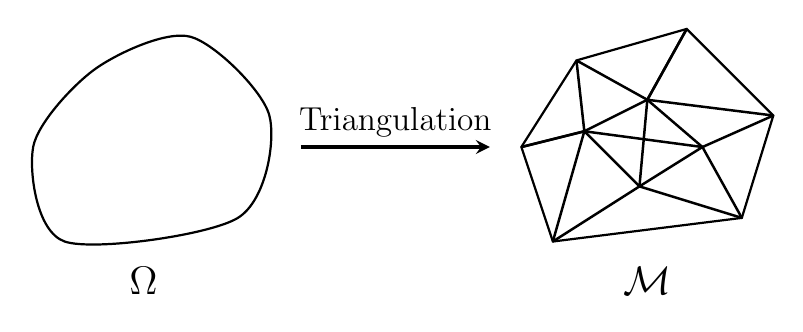
\begin{tikzpicture}[
        >=stealth,
        line width=0.9pt,
        every node/.style={font=\large}
    ]
    % Left: continuous domain Omega
    \begin{scope}[shift={(0,0)}]
      % Draw a smooth-ish domain
      \draw[thick]
        plot [smooth cycle, tension=0.5]
        coordinates {
          (0,0)
          (2.2,0.3)
          (2.6,1.6)
          (1.6,2.6)
          (0.4,2.2)
          (-0.4,1.2)
        };
      % Label
      \node at (1,-0.5) {\Large $\Omega$};
    \end{scope}
    
    % Middle arrow
    \begin{scope}[shift={(4.2,1.2)}]
        \draw[very thick,->] (-1.2,0) -- (1.2,0);
        \node[above] at (0,0) {Triangulation};
    \end{scope}
    
    % Right: triangulated mesh M
    \begin{scope}[shift={(6.2,0)}]
        % Outer polygon (approximation of Omega)
        \coordinate (A) at (0,0);
        \coordinate (B) at (2.4,0.3);
        \coordinate (C) at (2.8,1.6);
        \coordinate (D) at (1.7,2.7);
        \coordinate (E) at (0.3,2.3);
        \coordinate (F) at (-0.4,1.2);
        % Boundary
        \draw[thick] (A)--(B)--(C)--(D)--(E)--(F)--cycle;
        % Some interior points
        \coordinate (P1) at (1.1,0.7);
        \coordinate (P2) at (1.9,1.2);
        \coordinate (P3) at (1.2,1.8);
        \coordinate (P4) at (0.4,1.4);
        % Draw triangulation
        \draw (A)--(P1)--(B);
        \draw (B)--(P2)--(C);
        \draw (C)--(P3)--(D);
        \draw (D)--(P3)--(E);
        \draw (E)--(P4)--(F);
        \draw (F)--(P4)--(A);
        \draw (P1)--(P2)--(P3)--(P4)--cycle;
        \draw (P1)--(P3);
        \draw (P2)--(P4);
        % Label
        \node at (1.2,-0.5) {\Large $\mathcal M$};
    \end{scope}
    \end{tikzpicture}
    \caption{The triangulation $\mathcal{M}$ (the mesh) of $\Omega$. $\mathcal{M}$ is made up of $N$ nodes located at the vertices (corners) of the triangles.}
    \label{fig:triangulation}
\end{figure}